\documentclass[tikz,border=2pt]{standalone}
\usepackage{amsmath,amssymb}
\usepackage{tikz}
\usetikzlibrary{matrix}

\begin{document}
% The nonbasic variables (s_1, s_2 here) are set to zero; their columns carry the information
% of how z and the basic variables would change if one of them were raised.
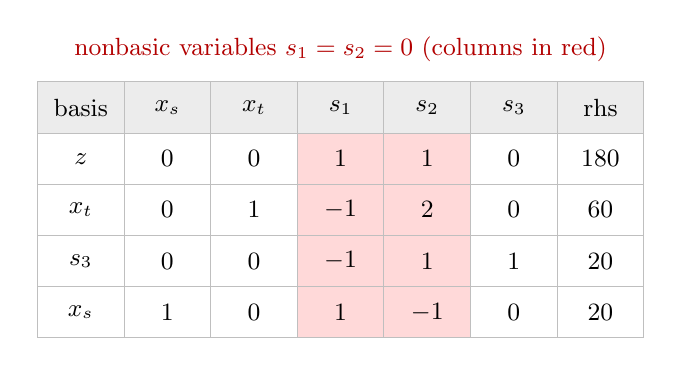
\begin{tikzpicture}[every node/.style={font=\small}]
	\matrix (T) [matrix of math nodes, nodes={minimum width=1.1cm, minimum height=6.5mm, anchor=center, draw=gray!50}, column sep=-\pgflinewidth, row sep=-\pgflinewidth] at (0,0) {
		|[fill=gray!15]| \text{basis} & |[fill=gray!15]| x_s & |[fill=gray!15]| x_t & |[fill=gray!15]| s_1 & |[fill=gray!15]| s_2 & |[fill=gray!15]| s_3 & |[fill=gray!15]| \text{rhs} \\
		z & 0 & 0 & |[fill=red!15]| 1 & |[fill=red!15]| 1 & 0 & 180 \\
		x_t & 0 & 1 & |[fill=red!15]| -1 & |[fill=red!15]| 2 & 0 & 60 \\
		s_3 & 0 & 0 & |[fill=red!15]| -1 & |[fill=red!15]| 1 & 1 & 20 \\
		x_s & 1 & 0 & |[fill=red!15]| 1 & |[fill=red!15]| -1 & 0 & 20 \\
	};
	\node[red!70!black, anchor=south] at (T.north) {nonbasic variables $s_1=s_2=0$ (columns in red)};
	\end{tikzpicture}
\end{document}
